\begin{frame}{3D Druck}
    \begin{minipage}[b]{.6\textwidth}
    \begin{figure}
        \centering
        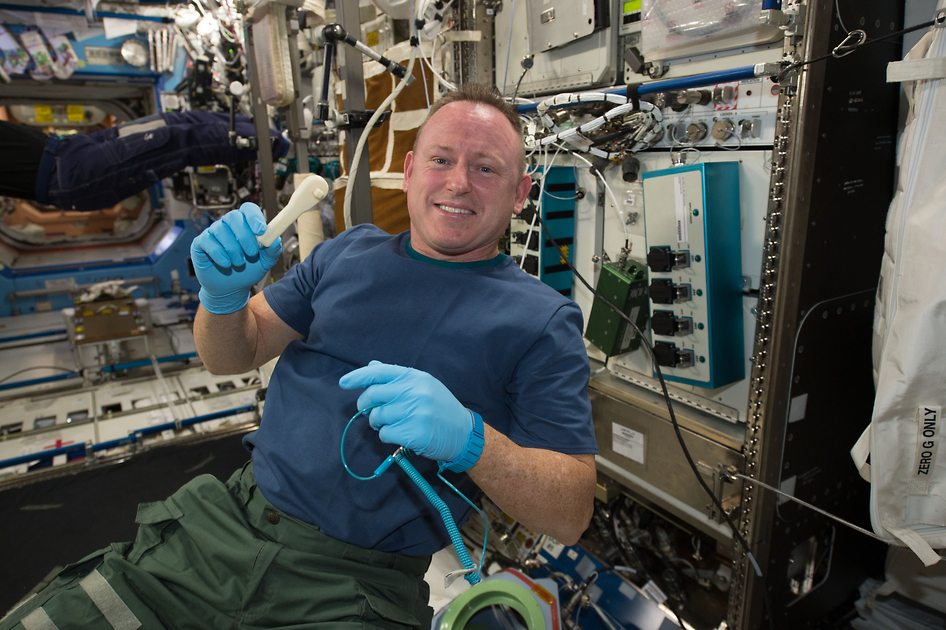
\includegraphics[width=190pt]{img_niklas/iss_wrench.jpg}
        \caption*{ISS Schraubenschlüssel}
        \label{fig:my_label}
    \end{figure}
    \end{minipage}
    \hfill
    \begin{minipage}[b]{.39\textwidth}
    \begin{block}{3D Drucker}
        \begin{itemize}
            \item Einsatzwecke
            \begin{itemize}
                \item Industrie
                \item Heimnutzung
                \item Forschung
            \end{itemize}
            \item Verschiedene Typen
            \begin{itemize}
                \item Ähnliche Arbeitsweisen
                \item Verschiedene Anforderungen
            \end{itemize}
            \item Funktionsweise
            \item Dateiformat STL
        \end{itemize}
    \end{block}
    \end{minipage}
    
\end{frame}

\begin{frame}{3D Drucker Typen}
    \begin{figure}[t]
        \centering
        \begin{minipage}[m]{0.49\textwidth}
        \begin{figure}
            \centering
            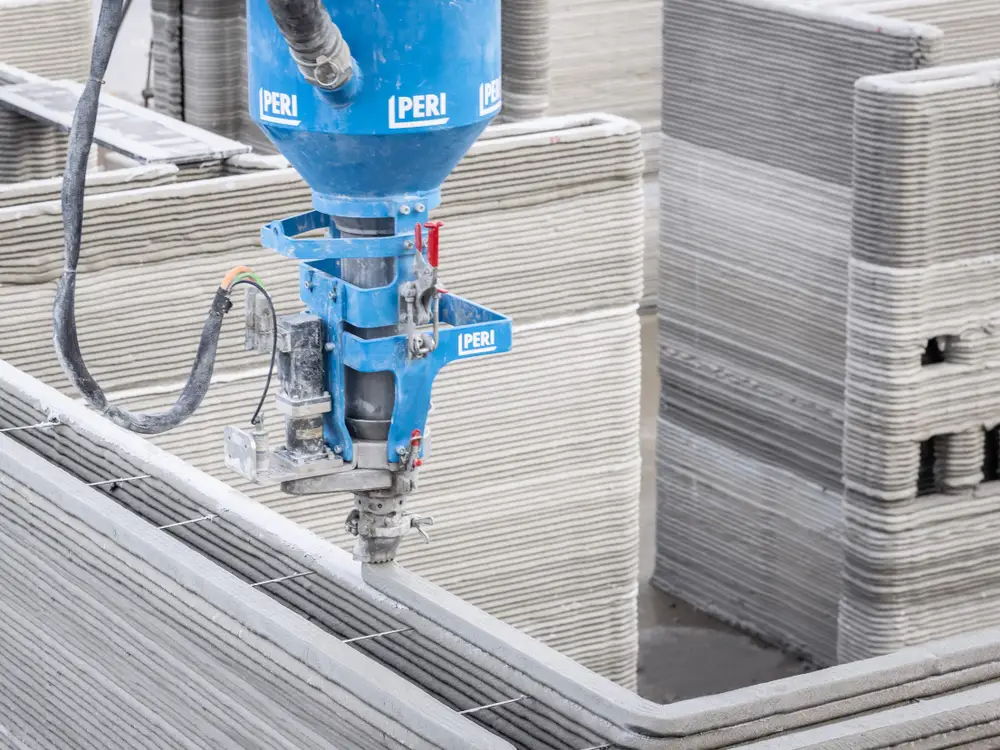
\includegraphics[height=90pt]{img_niklas/3dhouse.png}
            \label{fig:my_label}
        \end{figure}
        \end{minipage}
        \begin{minipage}[m]{0.49\textwidth}
         \begin{figure}
            \centering
            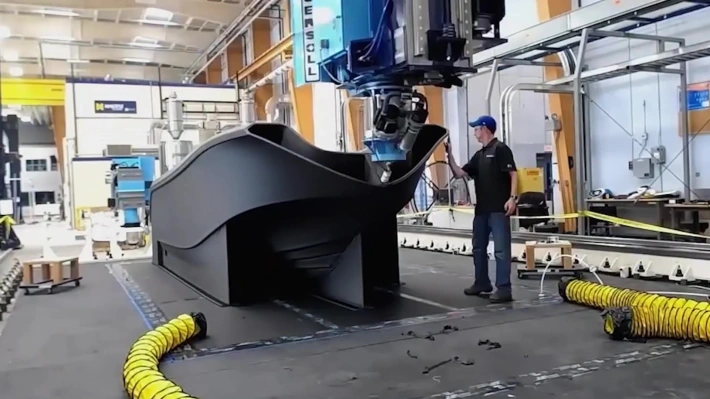
\includegraphics[height=90pt]{img_niklas/3dboat.png}
            \label{fig:my_label}
        \end{figure}
        \end{minipage}
    \end{figure}
    %%bottom
     \begin{figure}[b]
        \centering
        \begin{minipage}[m]{0.49\textwidth}
        \begin{figure}
            \centering
            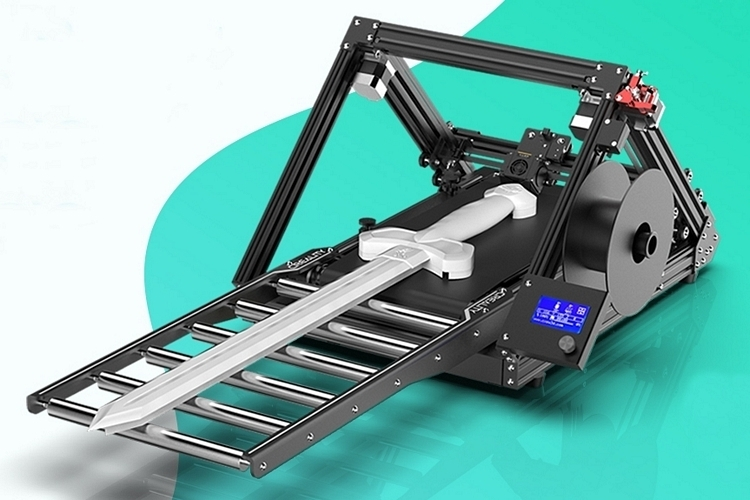
\includegraphics[height=90pt]{img_niklas/creality-cr30-3dprintmill-1.jpg}
            \label{fig:my_label}
        \end{figure}
        \end{minipage}
        \begin{minipage}[m]{0.49\textwidth}
         \begin{figure}
            \centering
            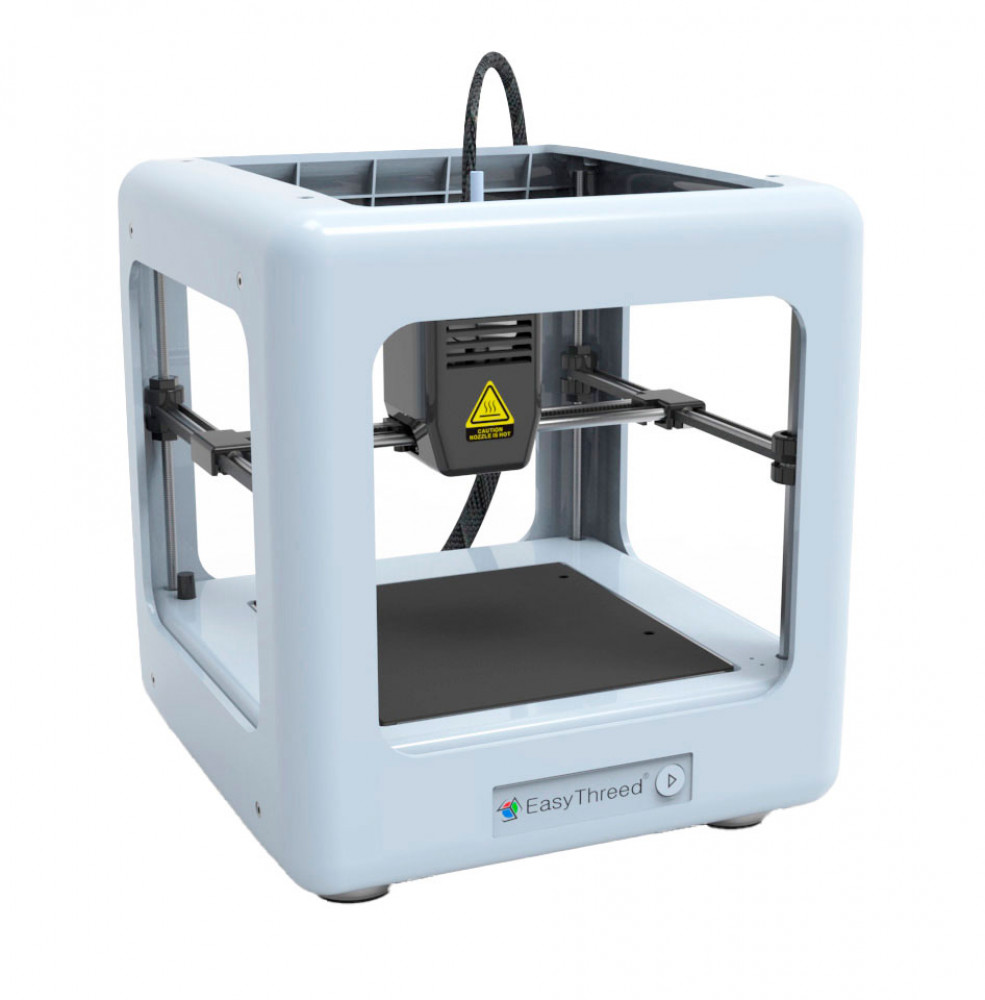
\includegraphics[height=90pt]{img_niklas/3d_printer2.jpg}
            \label{fig:my_label}
        \end{figure}
        \end{minipage}
    \end{figure}
    
\end{frame}

\begin{frame}{FDM vs SLA}
    \begin{minipage}[b]{.45\textwidth}
    \begin{figure}
        \centering
    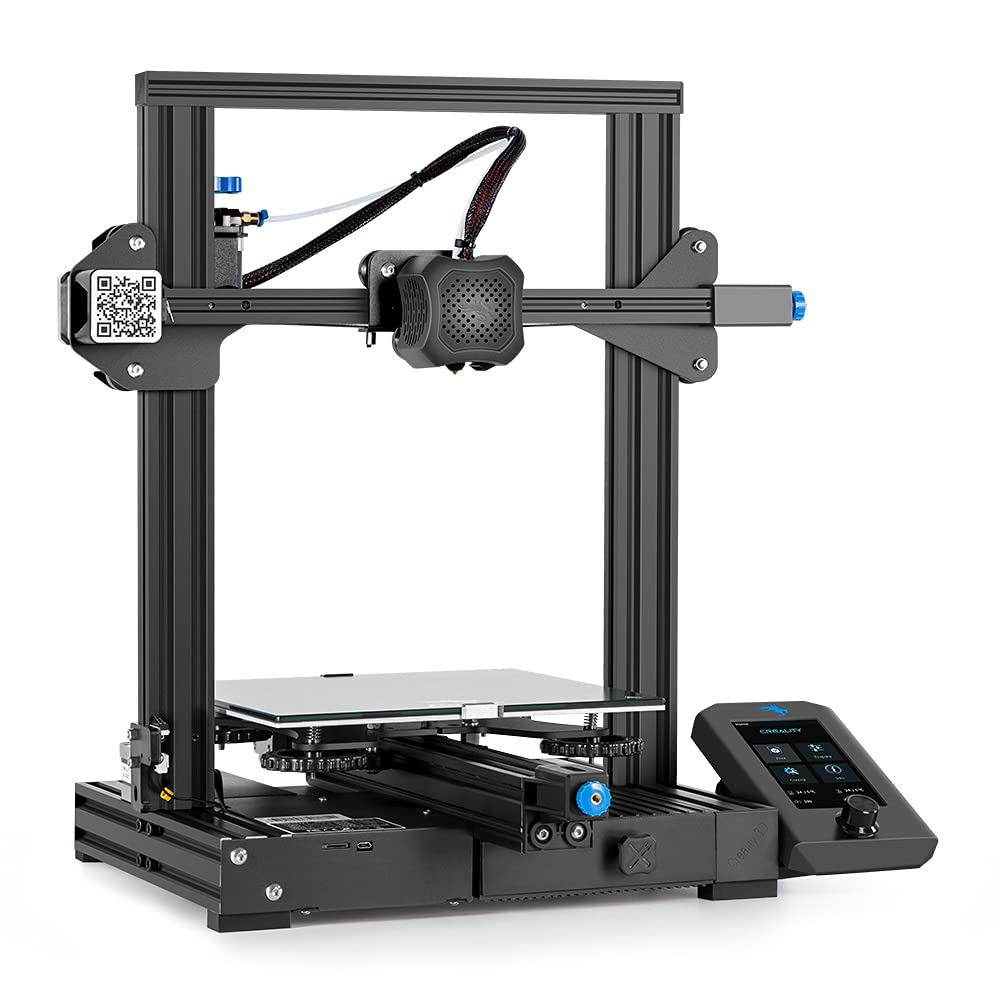
\includegraphics[width=150pt]{img_niklas/3d_printer.jpg}        
    \caption*{Fused Deposition Modeling (FDM)}
    \end{figure}
    \end{minipage}
    \begin{minipage}[b]{.45\textwidth}
    \begin{figure}[]
        \centering
        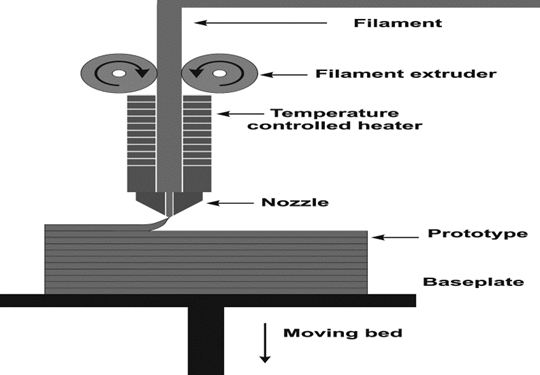
\includegraphics[width=150pt]{img_niklas/Schematic-of-an-FDM-3D-printer-Reproduced-with-permission-from-12.png}
        \caption*{FDM Funktionsweise}
        \label{fig:my_label}
    \end{figure}
    \end{minipage}
\end{frame}

\begin{frame}{FDM vs SLA}
    \begin{minipage}[b]{.45\textwidth}
    \begin{figure}
        \centering
        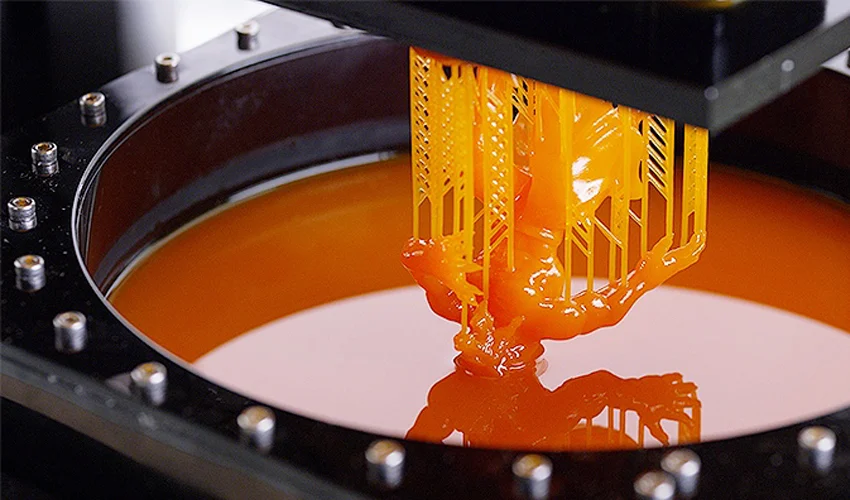
\includegraphics[width=150pt]{img_niklas/SLA_Technology-1.png}
        \caption*{Stereolithografie (SLA)}
        \label{fig:my_label}
    \end{figure}
    \end{minipage}
    \hfill
    \begin{minipage}[b]{.45\textwidth}
    \begin{figure}[]
        \centering
        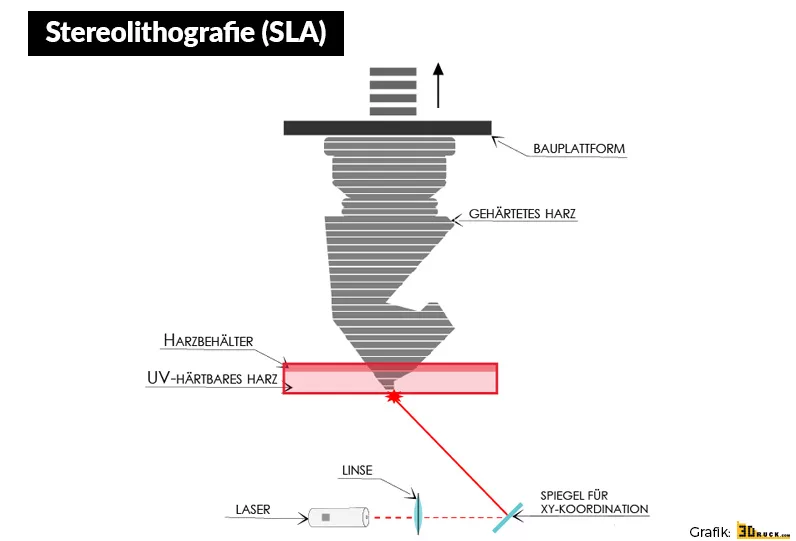
\includegraphics[width=180pt]{img_niklas/sla-stereolithografie-3d-druck.jpg.png}
        \caption*{SLA Funktionsweise}
        \label{fig:my_label}
    \end{figure}
    \end{minipage}
\end{frame}

\begin{frame}{Dateiformat STL}
    \centering
    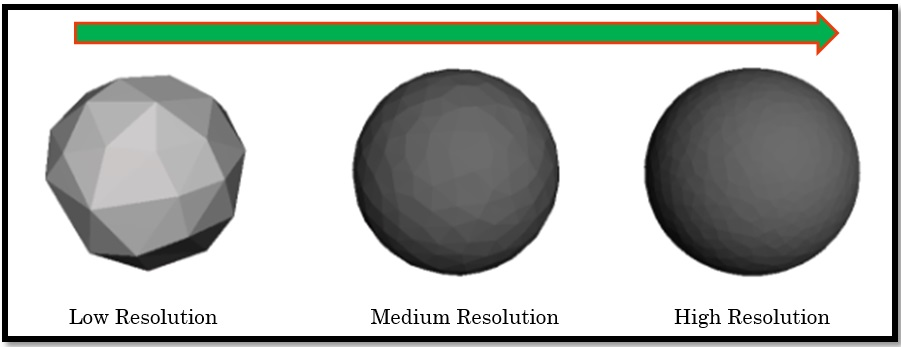
\includegraphics[width=300pt]{img_niklas/stl.jpg}
    \begin{figure}
        \centering
        \begin{minipage}[m]{0.3\textwidth}
        \begin{itemize}
            \item Standard Transformation Language
            \item Körper werden in Dreiecken unterteilt
        \end{itemize}
        \end{minipage}
        \begin{minipage}[m]{0.3\textwidth}
        \begin{itemize}
            \item Slicer macht aus STL Datei G-Code
            \item G-Code wird vom Drucker 'abgefahren'
        \end{itemize}
        \end{minipage}
        \begin{minipage}[m]{0.3\textwidth}
        \begin{itemize}
            \item Kompromiss zwischen Auflösung und Größe
        \end{itemize}
        \end{minipage}
    \end{figure}
    
\end{frame}